\subsection{Centered Parabolas on the Branches}
\label{sec:setup.quad.even}

We start by examining this piecewise quadratic model with centered parabolas.
For this, we set $a_L = a_R = 6$, $b_L = -\frac{3}{2}$, and $b_R = -\frac{9}{2}$ to keep the minimum in the center of the branches.
The parameters not fixed are $c_L$ and $c_R$.
They are both varied in the range $[0.25, 0.6]$.

This emulates the effect that $\chi_0$ has on branches $f_\A$ and $f_\C$.
Increasing $c_L$ increases the values on branches $f_\A$ and $f_\C$.
The effects of $E_0$ on branches $f_\B$ and $f_\D$ are lowering the value of the function at the left border of the branches and moving the minima on the branches to the left, as well as reducing the value of the function at the minima.
Decreasing $c_R$ does not have the same effects but rather lowers the values of the whole branches.
Scanning the periods of the stable cycles of the model under variation of the two parameters $c_L$ and $c_R$ results in \Cref{fig:setup.quad.even.period.full}.

\begin{figure}
	\centering
	\begin{subfigure}{0.4\textwidth}
		\centering
		\includegraphics[width=\textwidth]{21_Quadratic_mod1/2D_Period_Zoomed1/result.png}
		\caption{Full}
		\label{fig:setup.quad.even.period.full}
	\end{subfigure}
	\begin{subfigure}{0.4\textwidth}
		\centering
		\includegraphics[width=\textwidth]{21_Quadratic_mod1/2D_Period_Zoomed2/result.png}
		\caption{Zoomed}
		\label{fig:setup.quad.even.period.zoomed}
	\end{subfigure}
	\caption[2D scans showing periods of the even piecewise quadratic model]{
		2D scans showing the periods of the piecewise quadratic model with fixed parameters $a_L = a_R = 6$, $b_L = -\frac{3}{2}$, and $b_R = -\frac{9}{2}$.
		(a) Shows the full structure with parameters $c_L$ and $c_R$ being varied in the range $[0.25, 0.6]$ both.
		The red rectangle marks the parameter range of (b).
		The marked points in (b) are the parameter values for the cobwebs in \Cref{fig:setup.quad.even.cobwebs}
	}
\end{figure}

\begin{figure}
	\centering
	\begin{subfigure}{0.3\textwidth}
		\centering
		\includegraphics[width=\textwidth]{21_Quadratic_mod1/Cobweb_A/result.png}
		\caption{At point $A$}
		\label{fig:setup.quad.even.cobweb.A}
	\end{subfigure}
	\begin{subfigure}{0.3\textwidth}
		\centering
		\includegraphics[width=\textwidth]{21_Quadratic_mod1/Cobweb_B/result.png}
		\caption{At point $B$}
		\label{fig:setup.quad.even.cobweb.B}
	\end{subfigure}
	\begin{subfigure}{0.3\textwidth}
		\centering
		\includegraphics[width=\textwidth]{21_Quadratic_mod1/Cobweb_C/result.png}
		\caption{At point $C$}
		\label{fig:setup.quad.even.cobweb.C}
	\end{subfigure}
	\caption[Cobwebs of the even quadratic model]{
		Cobweb diagrams at three parameter values of $c_L$ and $c_R$ in the piecewise quadratic model with fixed parameters $a_L = a_R = 6$, $b_L = -\frac{3}{2}$, and $b_R = -\frac{9}{2}$.
		The parameter values are marked in \Cref{fig:setup.quad.even.period.zoomed}.
	}
	\label{fig:setup.quad.even.cobwebs}
\end{figure}

A phenomenon like in the original model could not be found here.
But something very similar happens on the border of these wings.
\Cref{fig:setup.quad.even.cobwebs} shows the cobwebs at the points marked in \Cref{fig:setup.quad.even.period.zoomed}.
At point $A$, there is one stable cycle with period 8.
This cycle is depicted in \Cref{fig:setup.quad.even.cobweb.A} and its symbolic sequence is $\A^3B\C^3\D$.
Point $B$ is in a parameter region, where 2 stable cycles coexist.
You cannot see this in the 2D scans above, since it only ever picks up on one cycle.
\Cref{fig:setup.quad.even.cobweb.B} shows the coexisting cycles at this border.
In contrast to the original model, the cycle that existed before in \Cref{fig:setup.quad.even.cobweb.A}, still exists alongside the new cycle with period 6.
The symbolic sequence of the new cycle is $\A^2\B\C^2\D$.

\todo{At point C?}

This is different from the dynamics in the original model in two ways.
First, the cycles before and after the area of coexistence have different periods.
And second, the cycles existing outside the area of coexistence still exist inside the area of coexistence.
In the original model, the cycles existing outside the area of coexistence would disappear at the border and new cycles would emerge inside this area.
Here, we simply observe two overlapping parameter regions which is something different from the original model.
